\section{Controlled experiments}
\label{sec:synthetic}
\subsection{Design and validation}
The synthetic experiment has known candidate accuracies, allowing genuine coverage and decision error to be measured. Candidate 0 has accuracy 0.4. Equal-quality cells set every candidate to 0.4; heterogeneous cells place the other candidates evenly over $[0.32,0.48]$ ($K=2$ has a single challenger at 0.48). On each independent question, with probability $\rho$ all candidates compare a shared $U\sim\mathrm{Uniform}(0,1)$ against their own accuracy; otherwise they compare independent uniforms. Thus
\begin{equation}
 \mathrm{Cov}(Y_j,Y_k)=\rho\{\min(\theta_j,\theta_k)-\theta_j\theta_k\},\quad j\ne k.
\end{equation}
Each marginal variance is $\theta_j(1-\theta_j)$, independently of $\rho$. For equal accuracies, pairwise correctness correlation equals $\rho$; for heterogeneous accuracies, $\rho$ is the mixture probability rather than the correlation itself.

The complete grid crosses $n\in\{16,32,64,128,256,512\}$, $K\in\{1,2,4,8,16,32,64,128\}$, $\rho\in\{0,0.5,0.9\}$, and quality-spread parameter $\{0,0.08\}$. Each of 288 cells has 20,000 independent repetitions, for 5.76 million whole-search experiments, with master seed 20261103. Each reported mean has a Monte Carlo standard error (MCSE); for rates the standard error is computed across independent event indicators. These uncertainties concern simulation error. All outcomes, including no-selection and small-gap cases, are retained.

An exact sufficient-count sampler avoids materializing every binary row while preserving the specified joint law. Distributional checks compare means and covariances with analytic values and test dependence endpoints. Exact binomial-maximum calculations independently check optimism, naive coverage, and simultaneous coverage in 48 independent equal-quality settings. Across 144 checks, the largest absolute simulation discrepancy is 3.651 MCSE. This validates the implementation against these references; it is not a universal proof of software correctness.

\subsection{Magnitude and drivers of score optimism}
Figure~\ref{fig:selection} isolates selection without genuine improvements: all candidates have accuracy 0.4. At $n=64$, $K=16$, and $\rho=0.5$, reuse overstates the selected accuracy by 7.705 percentage points on average (MCSE 0.035 pp). The ordinary nominal 95\% interval covers only 82.295\% of selected targets (MCSE 0.270 pp). Increasing the question count reduces sampling noise; increasing the bank size supplies more opportunities to select favorable noise. Shared errors reduce the effective diversity of these opportunities. These are conditional patterns under the specified data-generating mechanism, not a universal formula for real prompts.

The complete grid includes favorable cases as well as severe failures (Appendix~\ref{app:fullgrid}). At $n=512$, $K=128$, $\rho=0.9$, and spread 0.08, reused-score optimism is 1.031 pp (MCSE 0.015 pp). A clear quality advantage and strongly shared errors can therefore substantially reduce optimism. Across the prespecified grid, naive selected-candidate coverage ranges from 5.165\% to 97.525\%; these are empirical extrema, not simultaneous confidence limits for population extrema. In heterogeneous cells, changing $K$ also changes the true-quality grid, so the equal-quality cells provide the clean comparison for bank-size effects.

\begin{figure*}[t]
\centering
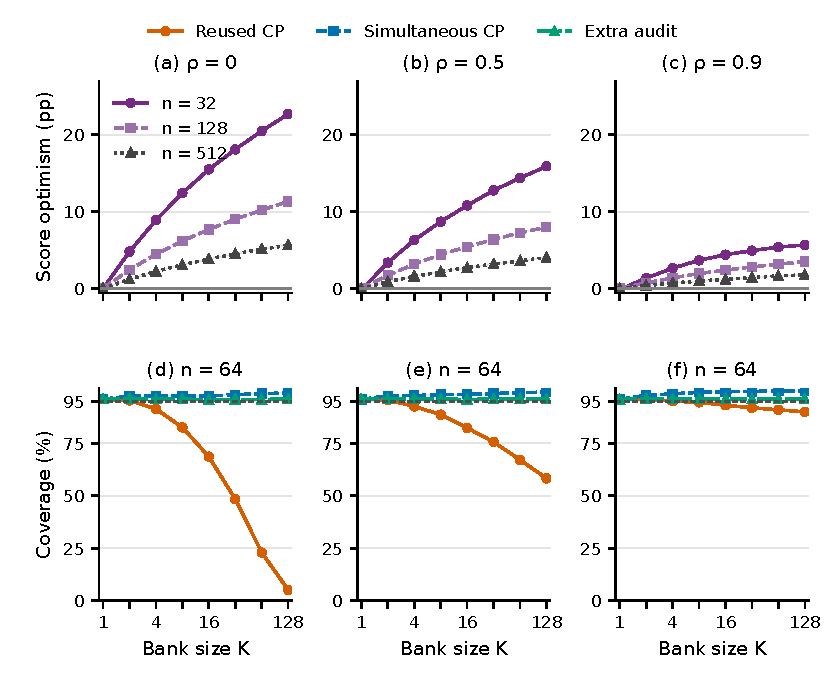
\includegraphics[width=\textwidth]{figures/synthetic-selection.pdf}
\caption{\textbf{Selection optimism and interval validity depend on bank size and shared errors.} All candidates have true accuracy 0.4. Columns vary correctness correlation $\rho$. Top: mean winning search score minus truth, for the labeled iid question counts $n$. Bottom: selected-target coverage of nominal 95\% CP intervals at $n=64$; the gray line marks 95\%. Simultaneous CP uses marginal error $0.05/K$. Extra audit scores the full-search winner on $n$ additional independent questions, costing $n$ calls beyond $nK$ search calls. Bands are marginal 95\% Monte Carlo intervals: mean $\pm1.96$ MCSE for optimism and exact binomial intervals for coverage, with 20,000 repetitions per cell. Some bands are narrower than markers. Correcting an interval leaves the reused point score unchanged.}
\label{fig:selection}
\end{figure*}

\subsection{Reliability, utility, and resource costs}
Table~\ref{tab:methods} illustrates two declared settings. In the equal-quality case, simultaneous coverage is 98.290\% (MCSE 0.092 pp), and an extra independent audit gives 95.835\% (MCSE 0.141 pp). Over the grid, their coverage estimates range from 95.145\% to 99.955\% and from 95.065\% to 97.605\%, respectively. CP discreteness and simultaneous correction both contribute conservatism; measured minima do not establish a simultaneous empirical guarantee. The mathematical guarantees depend on the fixed-bank iid assumptions in Section~\ref{sec:methods}.

\begin{table*}[t]
\caption{\textbf{Reporting protocols under two declared settings.} Entries are means (MCSE) from 20,000 independent repetitions. Bias is reported score minus the protocol's selected true accuracy. Width concerns nominal 95\% CP intervals; quality is the selected true accuracy. Bias and width are percentage points (pp), coverage and quality are percent. Both settings have $\rho=0.5$. Simultaneous CP retains the reused point score. Extra audit adds $n$ calls; question split preserves $n$ total questions; call split preserves $nK$ total calls. Parenthetical errors rounded to 0.000 are below 0.0005 in displayed units or exactly zero for constant truth. Full precision and counts accompany the source CSV.}
\label{tab:methods}
\centering
{\fontsize{8}{9}\selectfont\begin{tabular}{lrrrrr}
\toprule
Report & Bias (pp) & Coverage (\%) & Width (pp) & Quality (\%) & Calls \\
\midrule
\multicolumn{6}{l}{\textit{$n=64, K=16, \rho=0.5$; spread $0$}} \\
Reused CP & 7.71 (0.035) & 82.30 (0.270) & 25.39 (0.001) & 40.00 (0.000) & 1,024 \\
Simultaneous CP & 7.71 (0.035) & 98.29 (0.092) & 36.79 (0.002) & 40.00 (0.000) & 1,024 \\
Extra audit & 0.06 (0.043) & 95.84 (0.141) & 24.87 (0.005) & 40.00 (0.000) & 1,088 \\
Question split & -0.09 (0.062) & 95.25 (0.150) & 35.04 (0.010) & 40.00 (0.000) & 544 \\
Call split & 0.04 (0.043) & 96.03 (0.138) & 24.88 (0.005) & 40.00 (0.000) & 1,024 \\
\midrule
\multicolumn{6}{l}{\textit{$n=128, K=32, \rho=0.5$; spread $0.08$}} \\
Reused CP & 4.56 (0.027) & 88.33 (0.227) & 17.88 (0.001) & 46.52 (0.011) & 4,096 \\
Simultaneous CP & 4.56 (0.027) & 99.45 (0.052) & 28.03 (0.001) & 46.52 (0.011) & 4,096 \\
Extra audit & 0.01 (0.031) & 95.91 (0.140) & 17.81 (0.001) & 46.52 (0.011) & 4,224 \\
Question split & -0.04 (0.044) & 96.30 (0.134) & 25.24 (0.003) & 45.85 (0.016) & 2,112 \\
Call split & 0.04 (0.031) & 96.10 (0.137) & 17.81 (0.001) & 46.46 (0.012) & 4,096 \\
\bottomrule
\end{tabular}
}
\end{table*}

Reliable intervals need not be equally informative or equally costly (Figure~\ref{fig:budgets}). Simultaneous intervals avoid extra inference calls but widen. Extra auditing retains full-search quality and pays for additional observations. Reserving half the questions changes both the search winner and audit precision. At $n=128$, $K=32$, $\rho=0.5$, and spread 0.08, full search selects true quality 46.52\% (MCSE 0.011 pp), whereas the equal-question split selects 45.85\% (MCSE 0.016 pp). Its wider intervals and lower selected quality must be considered alongside its calibration. The call split spends fewer evaluations on every candidate to free calls for auditing only the winner; it permits more distinct questions than the question split. No method dominates all these criteria. Appendix~\ref{app:mse} reports MSE, which simultaneous intervals cannot change because they preserve the point score.

\begin{figure*}[t]
\centering
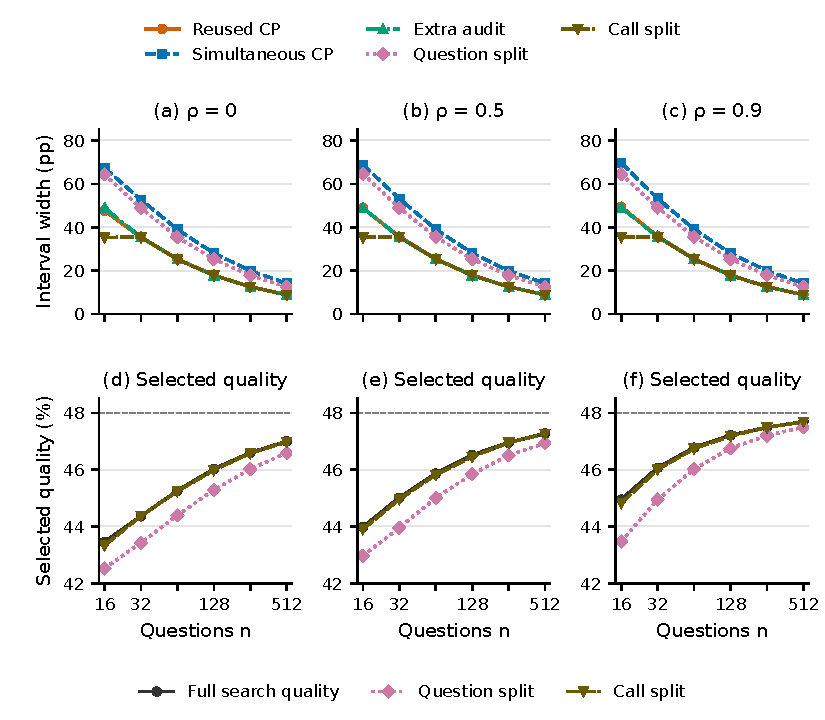
\includegraphics[width=\textwidth]{figures/synthetic-budgets.pdf}
\caption{\textbf{Reliable reporting trades uncertainty against search resources.} A bank of $K=32$ has a default accuracy 0.4 and other accuracies equally spaced over $[0.32,0.48]$. Columns vary shared-question mixture probability $\rho$, which is not exactly pairwise correlation for unequal means. Top: mean nominal 95\% interval width; bottom: mean selected true accuracy, with oracle 48\% dashed. Full search uses $nK$ calls. Extra audit adds $n$ calls and retains its winner. Question split reserves half the $n$ questions; call split uses $s=\lfloor nK/(K+1)\rfloor$ search and $h=nK-sK$ audit questions. Full-search methods share one quality curve. Bands are mean $\pm1.96$ MCSE over 20,000 repetitions. Width alone does not establish coverage, and split methods can select different targets.}
\label{fig:budgets}
\end{figure*}

\subsection{Consequences for a reported comparison}
Even the conservative interval-nonoverlap decision can fail after selection. At $n=512$, $K=128$, and independent equal-quality candidates, false superiority is reported in 9.890\% of repetitions (MCSE 0.211 pp), despite there being no true improvement. The frozen-pair 5\% error argument does not protect the data-selected pair. Appendix~\ref{app:decisions} shows the dependence on $K$ and $\rho$ and the simultaneous-interval comparison. This is evidence about this explicit decision rule, not a general false-discovery rate. Zero observed events in 20,000 repetitions would still permit a one-sided 95\% upper risk of approximately 0.015\%.
